\documentclass[12 pt]{paper}
\usepackage[utf8]{inputenc}
\usepackage[american]{babel}
\usepackage{paralist}%in order to enumerate inside a paragraph
%\usepackage[hyphens]{url}
\usepackage[colorlinks=true,linkcolor=blue,anchorcolor=black,citecolor=blue,filecolor=blue,menucolor=black,runcolor=red,urlcolor=blue]{hyperref} %to get hyperlinks
\usepackage{caption}
\usepackage{subcaption}
\usepackage{csquotes}
\newbox{\bigpicturebox}%to create collage 

\usepackage[style=apa,backend=biber]{biblatex}%to cite using apa7

\usepackage{geometry}%to change page specs
\usepackage{enumitem,varwidth}%image stuff
\usepackage[svgnames]{xcolor}%image stuff, so pictures are colored
%\usepackage{tikz}%image stuff
%\usetikzlibrary{shapes.geometric} %image stuff
%\usepackage{lmodern}
\usepackage{graphicx}%to follow the template from school
\usepackage{booktabs} %to follow the template from school
 \geometry{
	a4paper,
	left=25mm,
	top=25mm,
	right=25mm,
	bottom=25mm,
}

%to cite personal communications
\DeclareAutoCiteCommand{inline}{\mycite}{\cites}
\DeclareCiteCommand{\mycite}
{}
{\ifentrytype{personalcommunication}
	{\printnames{labelname} \mkbibparens{personal communication, \printdate}}
	{\mkbibparens{\usebibmacro{cite}}}%
}
{}
{}

\parindent24pt
%to follow the template from school


\graphicspath{ {./bilder/} } %where the pictures are
\addbibresource{MasterLibrary1.bib}
\title{%
Ditigization of early 1900's  postcards with aerial photo of Axvall }

\author{Sonia Lindblom \and Sicheng Yan}

\date{June 2021}

\begin{document}
\include{titlepage}

\section{Introduction}
This report of a digitization project of older postcards featuring, among others aerial photos of Axvall. -- insert dizitization in  bigger context ---. The aim of this project is to make the images available online to those interested in historical aerial photographs, for instance 
\begin{inparaenum}[i)]
	\item for geomorphology purposes \autocite[cf.][]{gomez2015}
	\item post card historical purposes
	\item history of the village
	\item military history
\end{inparaenum}


 
\section{Background}
Axvall is a village in Valle region, Skara Municipality, Väster Götaland county in Sweden. It was formerly a municipality itelsef, with railway station, mayor's office and other functions as well a big sanatorim, Stora Ekbergs Sanatorium. One proeminent part of Axvall's history is the housing of at most three military regments \autocite[]{broden2021} broden2021). One of them, Skarborgs regemente trained in Axevalla hed beteween 1696 and 1913 \autocite{frykmer1992}. The other two are reported by \textcite{broden2021}, Väster Götalands regemente I6 up to 1927 and Livhusararna K3 up to 1905. It is hard to determine what contributed to the end of the railway activity. Howevehandlarer it is closely realted to the extinsion of the military trainings on Axevalla hed, the extinsion of the beer brewery and so on. According to \textcite[]{broden2021} Axevalla hed was of military interest though up to the middle 1980's.

The postcards that are part of this project were inherited by two sibilings, Birgit and Lars Lindblom. The majority of them, were acquired in the 1936 as part of the inventory together with the buying of Ivar Larssons livs, a local grocery store in Axvall, as it was told by \autocite[]{Lars}. The process of creating this project was intense and brought much understanding about digitization of cultural heritage as it is reported in the following sections. 

\section{Methodological work}%this has to have about 1300 words)
\subsection{Selection of the material}

The postcards were in shoeboxes without any systematization. Some of them were bound with rubberbands in bunts of 20. The conditions varied from untouched cards to others played with by kids who painted on with crayon. They were them placed in acidic free plastic boxes and grouped in categories such as hospital, housing, aerial photographs and so on, separated with laminated folders. This was important to make sure all the cards that fit the chosen category were found and taken care of.
 
The aerial photographs were of major interest since among them there were cards  which were forbiden to be distributed due to restrictions from the Swedish Army. Since aerial photographs taken before 1950's are free to publish \autocite[][kap. 3, 3§]{lantm2018}, we decided that digitizing those images would be a good contribution for the history of Axvall. Further investigation revealed though that a photo that has been restricted before by is not included in the exception in \textcite{lantm2018}. We have applied for a new assessment from Swedish Army, and the images were asessed in the end of May 2021 by a Swedish Army official. We got verbal authorisation and a promise of a written document, which had though not come before the deadline for the assignment. 

Since the cards had been assessed before by the Swedish army and we have access to the original letter containing their decision, we considered it relevant to include the letter in the collection and to make sure the cards with the stamp of approval (two of them) were the ones selected for digitizing as it can be of historical interest. 
\subsection{Metadata}

\subsection{Image capture}

\subsubsection{Preparation phase}
The process of image capture might have been one of the most bothersome since we wanted to make sure we followed the standards determined by the Swedish Kungliga biblioteket. We sought creating a fixed photographic environnment following the recommendations in \textcite[]{dgf1216} and \textcite[part 3]{kronlund2021p3} with neutral background in light gray fabric an a static shelf (figure \ref{baset}) where the camera was placed facing down the motifs (180 $ ^{\circ} $).  Daylight was isolated with the help of two blackout curtains to come close to the standards in iso 3664 \autocite[cf.][]{johansson2021}. A light tent was used to assure homogeneus artificial illumination.  %
%ref light tent https://digital-photography-school.com/how-to-use-a-light-tent-for-small-product-photography/



\begin{figure}[!htb]
	\centering
	\caption[short:]{Image capture booth with a light tent}
	\fbox{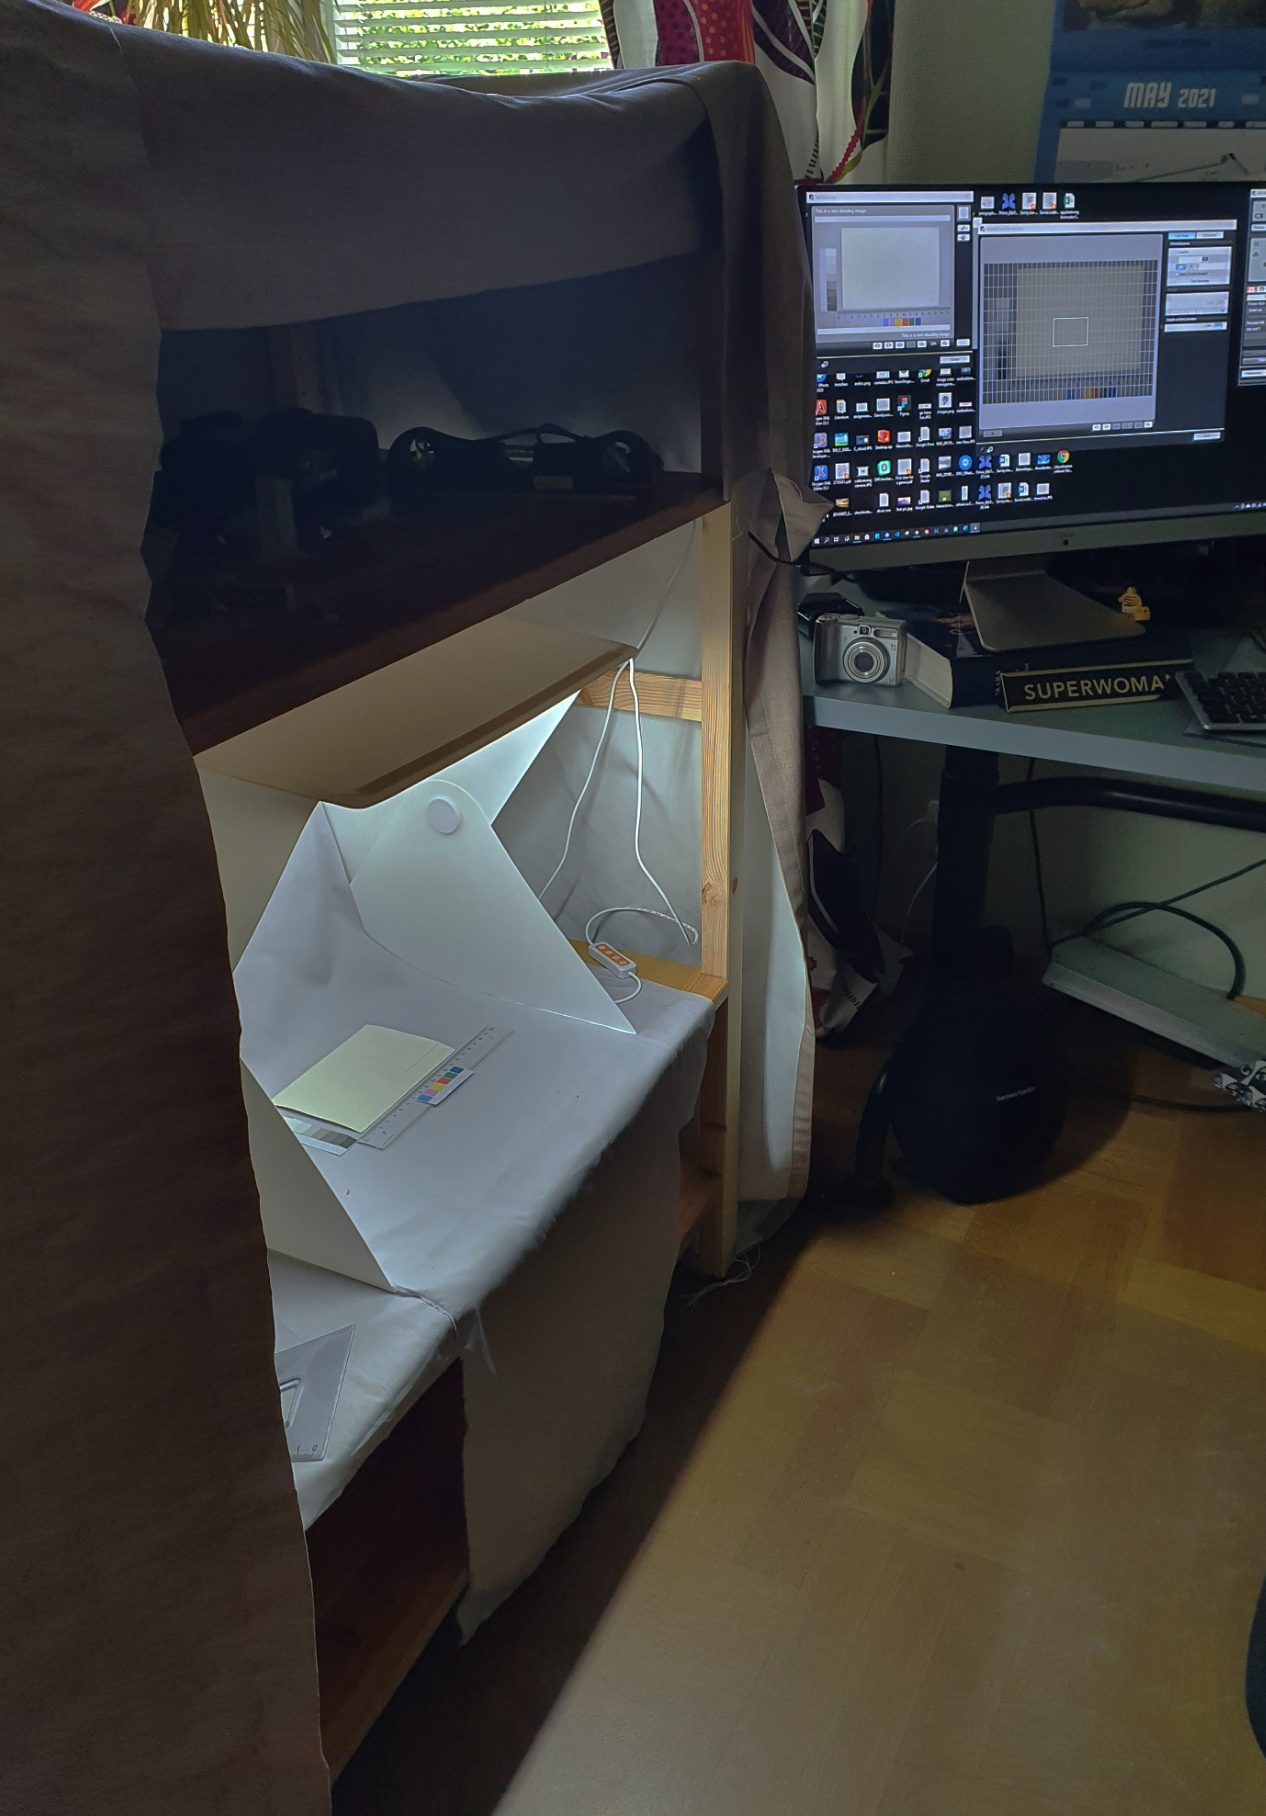
\includegraphics[width=0.5\linewidth]{baset.jpg}}
	\label{baset}
\end{figure}

Two color rulers, a gray scale and one colored,  were manufactured with the help of sample color pallets from NCS which was then translated to RGB with the help fo w3schools \autocite[]{w3}. The monitor was calibrated with the help of \textcite[]{koch2007}. 


\begin{figure}[!htb]
	\centering
	\caption[short:]{Image capture booth with a light tent}
	\fbox{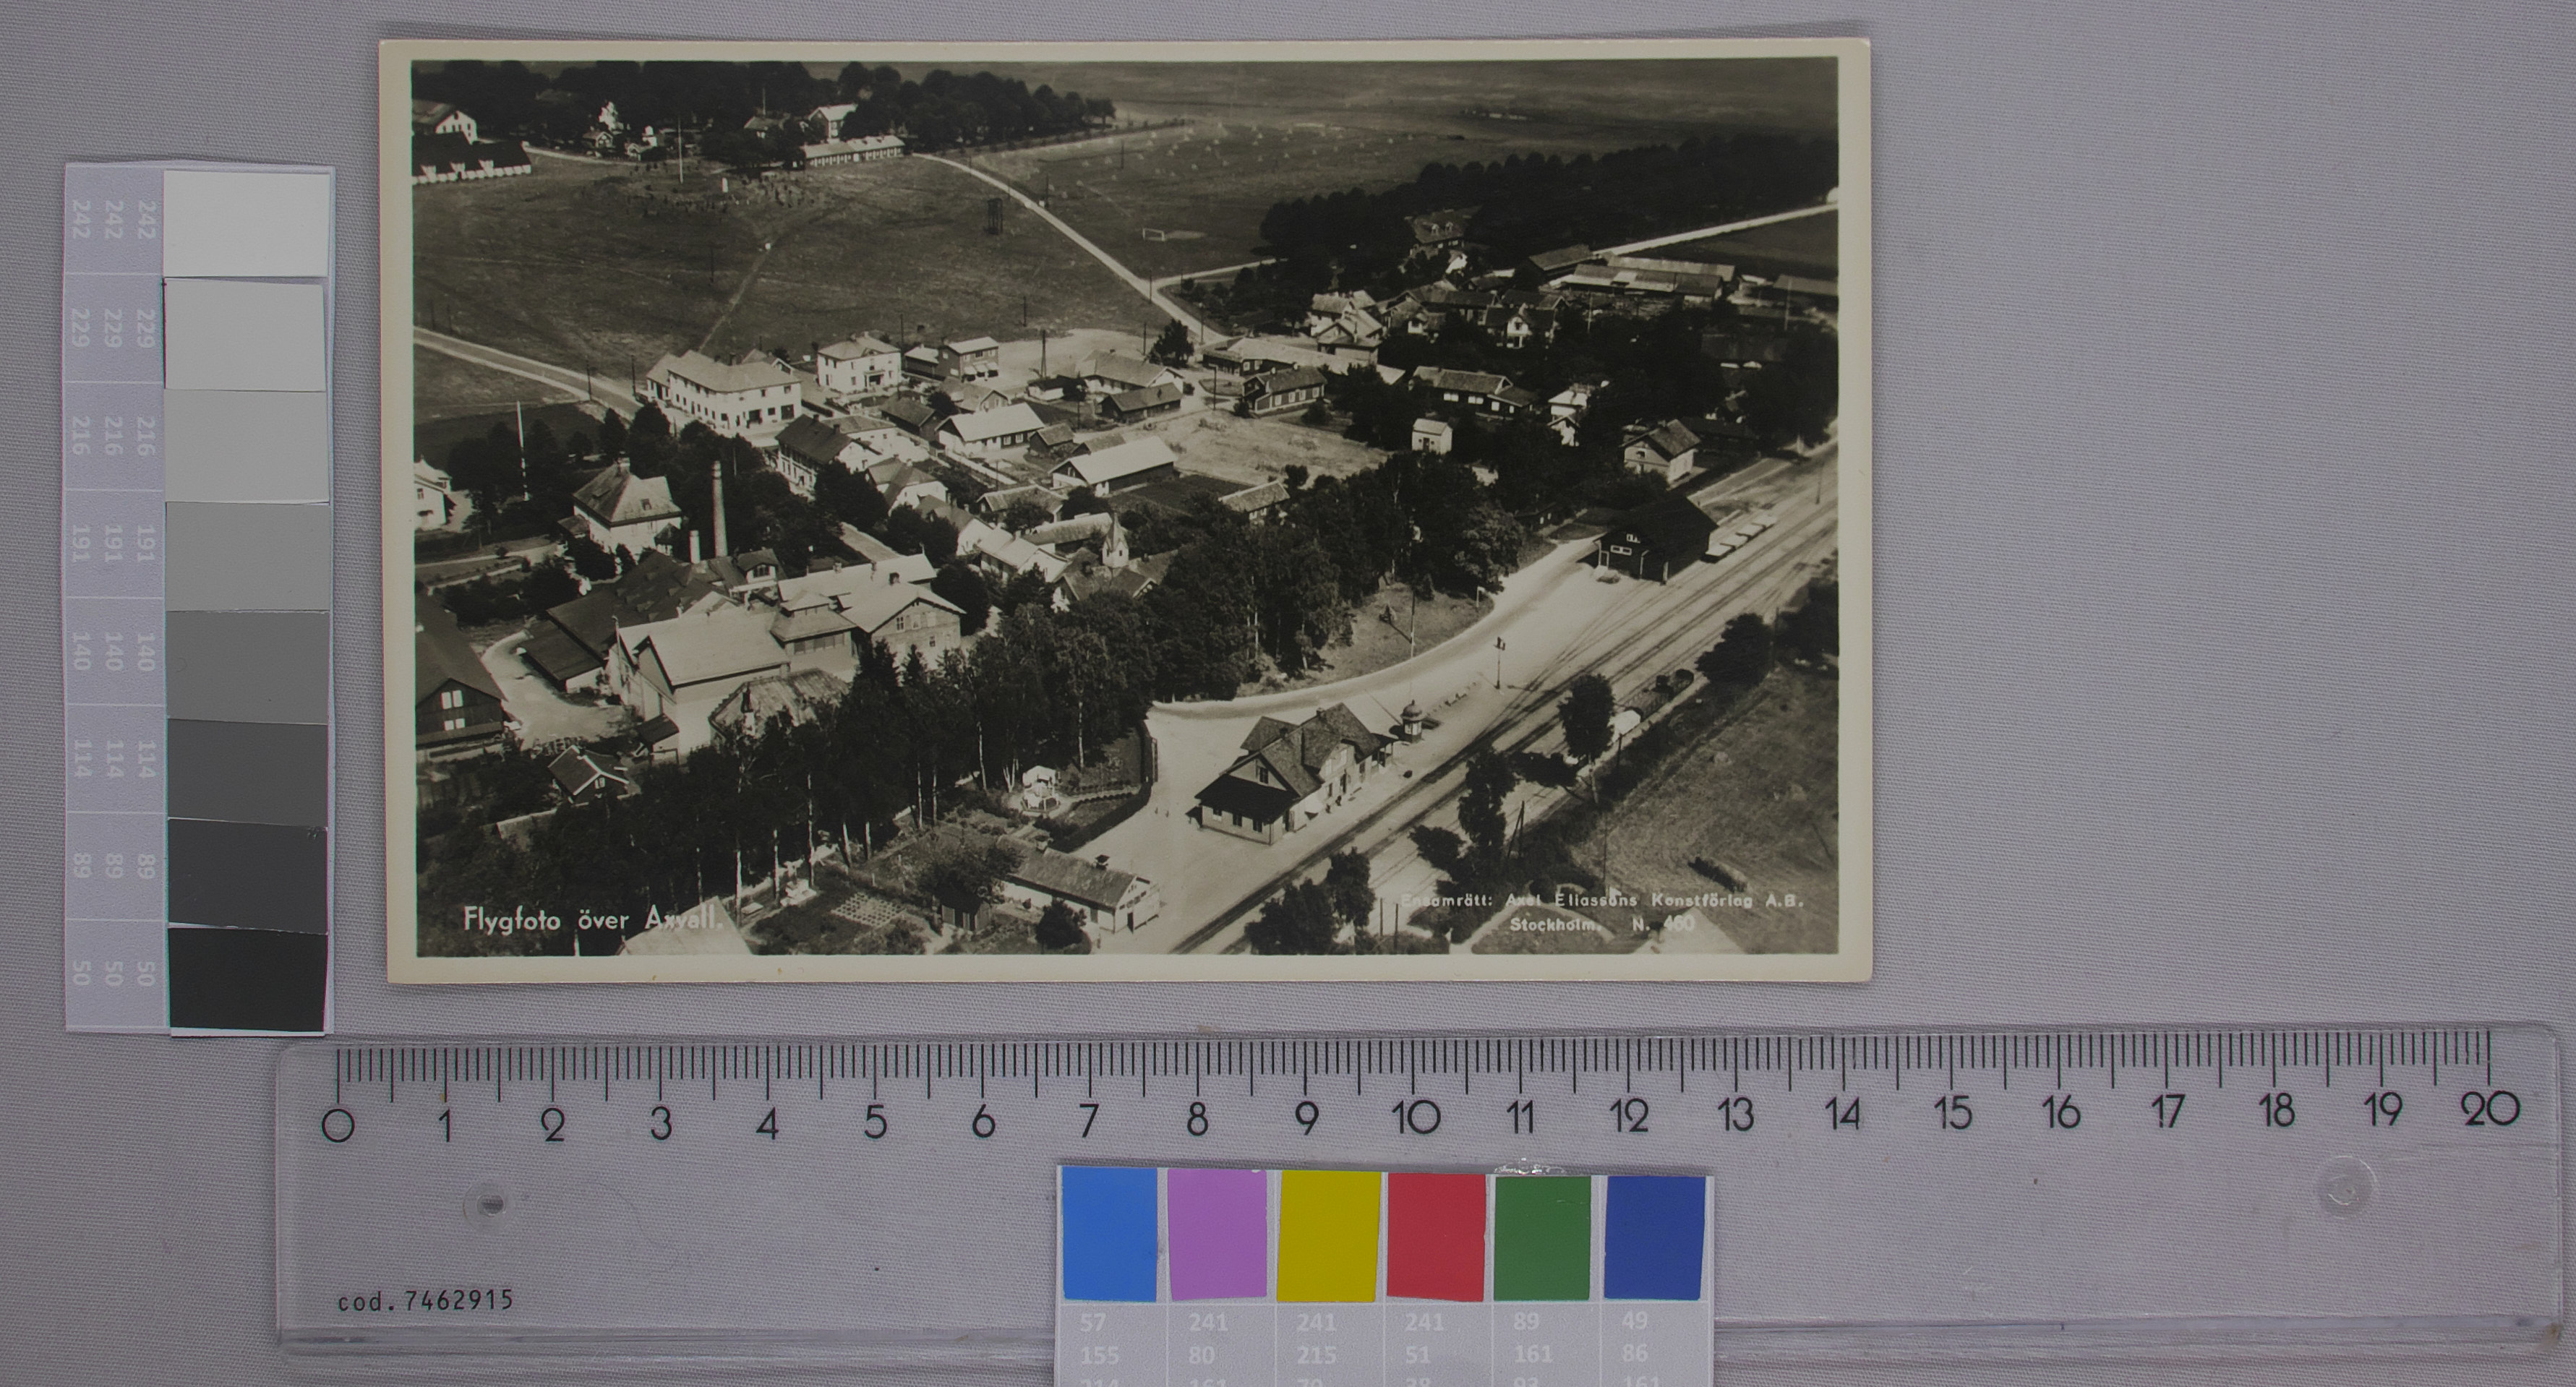
\includegraphics[width=0.5\linewidth]{colorrulerAfterfixing.jpg}}
	\label{ruler}
\end{figure}



\subsubsection{Digitization}

  The camera used for the final shooting is a Panasonic Lumix GX80. The images were captured remotely with the help of Panasonic Image App. make sure the camera settings and distance from the motifs were always the same. 
  
  The shooting was done with manual settings, since the authomatic ones caused changes according to the motif - if more or less white on them, for example. Figure \ref{tekniskMetatada}, shows the camerara settings, which is the same for every image.
  
  
  \begin{figure}[!htb]
  	\centering
  	\caption[short:]{Metadata from images, as shown in "properties" from windows explorer.}
  	\fbox{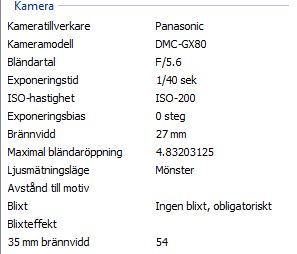
\includegraphics[width=0.4\linewidth]{tekniskMetatada.jpg}}
  	\label{tekniskMetatada}
  \end{figure}
  
 The light temprerature was set to 5000 Kelvin;
 
 

\subsection{.... platform}% Or something like webdesign


\subsection{Distribution of labor}

\begin{table}
	
	\caption{}
\end{table}
\section {Critical Analysis}


\subsection{Ethical issues and other considerations}

In the process of distribution, we planned making a webpage that is hosten on github. Some ethical issues \autocite[cf.][]{manzuch2017} arouse when planning the publication. The postcards were lent to us by their current owner, Lars Lindblom and for that reason, we cannot authorize the copy and redistribution of them without his consent - some of them might have commercial value. The selection process included sorting out every card from the huge amount of different cathegories, for that we sough consent from the  current owner. We have considered engaging the local community \autocite[cf.][]{hss2020, manzuch2017} in getting information about the places depicted in the photos. However, we face two constraints (i) the long process of assorting the cards and (ii) the uncertainty of which cards were possible to publish. 

When it comes to copyright issues, since the cards date from at latest

\section{Conclusions}
The objective of this project was to digitize postcards from a village in Sweden. The process included a great amount of learning. Much work was done in the preparation phase that included separating the cards to be used from a large amount of other postcards. We also had intensive contact with authorities (Lantmäteriet and Swedish Army) in order to be sure we were able to use every card in the project. 


\newpage

%\bibliographystyle{apacite}
%\bibliography{../../../MasterLibrary.bib}
\printbibliography


\end{document}


